\section*{Источники и решения}

\subsection*{Укрепление сетки}

Эту интересную (и, возможно, практически полезную) головоломку подкинул мне геометрический гуру Боб Коннелли из Корнелла; она основана на работе Этана Болкера и Генри Крапо \cite{bolker-crap}.


\begin{figure}[ht!]
\centering
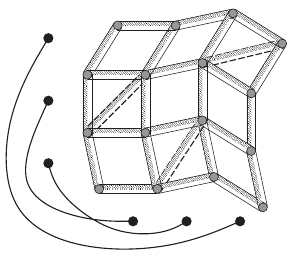
\includegraphics[scale=1]{pics/lattice2}
\caption{Недоукреплённая сетка и её граф.}
\label{pic:lattice2}
\end{figure}

\begin{figure}[b!]
\centering
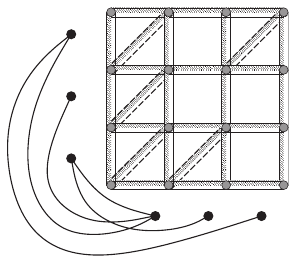
\includegraphics[scale=1]{pics/lattice3}
\caption{Полностью укреплённая сетка и её граф.}
\label{pic:lattice3}
\end{figure}

Задачу полезно перевести на язык графов, но сделать это не самым очевидным образом (не нужно смотреть на граф с вершинами в сочленениях стержней).
Для этого предположим, что скобы установлены;
рассмотрим граф $G$, вершины которого соответствуют строкам и столбцам из квадратов.
Каждое ребро в $G$ соответствует строке и столбцу, пересекающимся по закреплённому квадрату, так что число рёбер в $G$ равно числу скоб.
Сетка с рис. \ref{pic:lattice1}, показана снова на рис. \ref{pic:lattice2}, но уже с её графом.

Если строка и столбец смежны в $G$, то все вертикальные стержни в сей строке оперпендикулярны горизонтальным стержням в сём столбце.
Если $G$ --- связный граф (то есть существует путь от любой вершины к любой другой), то все горизонтальные стержни должны быть перпендикулярны всем вертикальным.
Таким образом, все горизонтальные стержни параллельны друг другу, и аналогично для вертикальные.
Теперь ясно, что сетка жёсткая.

С другой стороны, предположим, что граф несвязен.
Пусть $C$ --- его компонента, то есть связанным фрагмент $G$, который не имеет рёбер к остальной части $G$.
Тогда ничто не мешает любому вертикальному стержню в строке $C$ или любому горизонтальному стержню в столбце $C$ сгибаться относительно других стержней в сетке.
Таким образом, жёсткость в точности означает то, что $G$ связен.
Поскольку $G$ имеет $2n$ вершин, если он связен, то имеет как минимум $2n - 1$ ребро
(если это для вас новость, то докажите это индукцией по числу вершин).
Следовательно, чтобы сделать сетку жёсткой, нужно как минимум $2n - 1$ скоб.

Однако обратите внимание скобы нельзя ставить где попало.
На рисунке 21 показана полностью закреплённая сетка $3 \times 3$ и её граф.
Попробуйте подсчитать число способов сделать сетку $3 \times 3$ жёсткой с минимальным числом (пятью) скобами.
Теорема теории графов (о том, что у каждого связного графа есть связный подграф, называемый остовым деревом, с минимальным числом рёбер) говорит нам, что если более чем $2n - 1$ квадратов закреплены и сетка жёсткая, то существуют способы удалить все, кроме $2n - 1$ скоб, сохранив жёсткость.

\subsection*{Путешествие по острову}

Вариант этой головоломки был взят на веб-страницу «The Puzzle Toad» с упомянутой выше книги «Московские математические олимпиады» Г. А. Гальперина и А. К. Толпыго \cite{galperin-tolpygo}.

Между перекрёстками текущее состояние Алоисия можно охарактеризовать тройкой, состоящей из ребра, на котором он находится, направления движения по нему и типа последнего поворота (вправо или влево).
Поскольку таких троек конечное число, настанет момент, когда Алоисий впервые попадёт в одну и ту же тройку; это может произойти только на его стартовом ребре!

\begin{addedbytheeditors}
\textbf{Редакторам:} Наверно стоит добавить пару слов об обратом ходе.
\end{addedbytheeditors}


\subsection*{Провода под Гудзоном}

Вариацию головоломки пропагандировал Мартин Гарднер, иногда её называют задачей Грэма --- Нолтона.
Для электриков это задача идентификации проводов.
В версии Гарднера можно было замыкать любое число проводов на любом берегу и также проверять их на любом берегу.
Следующее решение было предложено Роландом Спрэгой в его книге \cite{sprague} и также в недавней статье трёх молодых специалистов по информатики: Навина Гойала, Сачина Лодхи и С. Мутукришнана \cite{goyal-lodha-muthukrishnan}.
Оно удовлетворяет нашим дополнительным ограничениям и требует только две операции на каждом конце (таким образом, потребуется три переправы через реку, не считая дополнительных переправ для размыкания проводов перед их использованием).
Однако решение не единственное, поэтому даже если ваше трёхпереправное решение отличается, оно может оказаться не хуже.

Обозначим через $w_1$, $w_2, \dots, w_{50}$ провода на западном берегу,
и $e_1, \dots, e_{50}$ на восточном. %??? n>50
При первом посещении западного берега, соединим $w_1$ с $w_2$, $w_3$ с $w_4$, $w_5$ с $w_6$ и так далее, но не будем соединять послднюю пару $w_{49}$ и $w_{50}$.
Затем проверим пары концов проводов на восточном берегу, пока не обнаружим все пары.
Например, мы можем обнаружить, что соединены $e_4$ с $e_{29}$, $e_2$ с $e_{15}$, $e_8$ с $e_{31}$ и так далее, а в конце концов, что $e_{12}$ и $e_{40}$ остались без пары.
Затем мы едем на западный берег, рассоединяем все пары и соединяем $w_2$ с $w_3$, $w_4$ с $w_5$ и так далее, оставив $w_1$ и $w_{50}$ без соединения.
Далее, мы проверяем пары на восточном конце, пока не обнаружим все соединённые пары концов.
Продолжая пример, пусть $e_{12}$ соединён с $e_{15}$, $e_{29}$ с $e_2$, и $e_4$ с $e_{31}$, а $e_{40}$ и $e_8$ остались без пары.

Удивительно, но этой процедуры достаточно для идентификации всех проводов!

Заметим, что один восточный конец провода, который был спарен в первый раз, но не во второй (в нашем примере это $e_8$), должен соответствовать $w_1$.
Восточный конец провода, с которым $e_8$ был спарен в первый раз (у нас это $e_{31}$), следовательно, должен соответствовать $w_2$.
Но тогда $w_3$ должен соответствовать восточному концу провода, с которым $e_{31}$ был спарен во второй раз, а именно $e_4$.
Продолжая таким образом, мы находим, что $w_4$ соответствует $e_{29}$ (паре $e_4$ на первом круге), $w_5$ соответствует $e_2$ (паре $e_{29}$ на втором круге) и так далее.
В конце концов мы видим, что $w_{50}$ соответствует $e_{40}$.

Если бы число проводов (скажем, $n$) было нечётным, мы оставили бы только $w_n$ вне пар в первый раз, а $w_1$ во второй раз, и всё сработает примерно так же.

\begin{addedbytheeditors}
Заметим, что задача не разрешима в случае $n=2$.
\end{addedbytheeditors}


\subsection*{Жуки на четырёх прямых}

Эту головоломку мне подкинул Мэтт Бэйкер из Технологического института Джорджии.
Иногда её называют \emph{задачей четырёх путешественников};
её можно увидеть на веб-сайте «Cut the knot» \cite{cut-the-knot}.

В наиболее изысканном решении, которое мне известно, требуется, подняться из плоскости в пространство, добавив ось времени.
Предположим, что каждая пара жуков встречается, кроме (возможно) третьего и четвёртого.
Проведём ось времени перпендикулярно плоскости с жуками, и пусть $g_i$ будет графиком $i$-го жука в пространстве.
Поскольку каждый жук ползёт с постоянной скоростью, каждый такой график является прямой;
его проекция на плоскость с жуками --- это та самая прямая, по которой ползёт соответственный жук.
Заметим, что два жука встречаются тогда (и только тогда) когда их графики пересекаются.

Прямые $g_1$, $g_2$ и $g_3$ находятся в одной плоскости, так как они попарно пересекаются.
Tо же самое относится и к тройке  $g_1$, $g_2$ и $g_4$.
Следовательно, все четыре графика лежат в одной плоскости прямых $g_1$ и $g_2$.
Конечно же $g_3$ и $g_4$ не параллельны, ведь не параллельны их проекции.
Таким образом, эти две прямые пересекаются в своей плоскости,
а это значит, что третий жук обязан встретить четвёртого.

\subsection*{Вменяемые мыслители}

Эта головоломка предложена Сашей Разборовым из Института перспективных исследований;
с его слов я знаю, что она была кандидатом на Международную математическую олимпиаду, однако была отвергнута как слишком сложная.
Она была рассмотрена и решена в статье Э. Голеса и Х. Оливоса \cite{goles-olivos}.

Чтобы доказать, что мнения установятся или будут переключаться каждую вторую неделю, будем думать о каждом знакомстве между как о паре стрелок, по одной в каждом направлении.
Назовём стрелку \emph{обиженной}, если мнение гражданина вначале стрелки отличается от мнения гражданина в конце стрелки на \emph{следующей неделе}.

Рассмотрим стрелки, выходящие от гражданина Клайда на неделе $t - 1$, во время которой (скажем) Клайд выступает за торговый центр.
Предположим, что из них $m$ обиженных.
Если Клайд все ещё (или снова) за торговый центр на неделе $t + 1$, то число $n$ обиженных стрелок, указывающих на Клайда на неделе $t$, будет точно равно $m$.

Однако, если Клайд против торгового центра на неделе $t + 1$, то $n$ будет строго меньше $m$, так как большинство его друзей были против торгового центра на неделе $t$.
Следовательно, большинство стрелок от Клайда были обиженными на неделе $t - 1$, а теперь только меньшинство обиженных стрелок направлены к Клайду на неделе $t$.

Всё это остаётся также верным и если Клайд был против торгового центра на неделе $t - 1$.

Но вот какое дело: каждая стрелка начинается у кого-то на неделе $t - 1$ и заканчивается у кого-то на неделе $t$. Таким образом, общее число обиженных стрелок не может увеличиваться между неделями $t - 1$ и $t$, и, оно будет строго уменьшаться, за исключением одного случая --- когда каждый гражданин имел такое же мнение на неделе $t - 1$, как и на неделе $t + 1$.

Однако, общее число обиженных стрелок в данную неделю не может бесконечно уменьшаться и в конечном итоге должно достичь некоторого числа $k$, с которого оно никогда не опустится.
В этот момент каждый гражданин либо сохранит своё мнение навсегда, либо будет менять его туда-сюда каждую неделю.

Задачу можно значительно обобщить, например, добавив веса к вершинам (что означает, что мнения некоторых граждан более ценны, чем мнения других), разрешив петли (можно учитывать своё собственное текущее мнение), разрешив механизмы разрешения конфликтов и даже разрешив различные пороги для смены мнений в пользу торгового центра и против него.

\subsection*{Лемминг на шахматной доске}

Эту замечательную головоломку придумал Кевин Пурбху, ещё будучи старшекласником в Торонто.
С тех пор Пурбху защитил диссертацию по математике в Университете Калифорнии в Беркли;
сейчас он постдок в Университете Британской Колумбии
и занимается чем-то под названием \emph{тропическая геометрия}.
Сам я узнал головоломку от Рави Вакилома, из Стэнфордского университета.

Лемминг действительно обречён.
Один из способов понять это (обнаруженный независимо Вакилом и мной) --- представить, что лемминг может перемещаться на любую соседнюю клетку, но должен повернуться в направлении стрелки, которую он там обнаружит.
Далее, лемминг не может повернуться на 360°, обойдя цикл;
если бы он мог, то можно уменьшать цикл, на котором он это делает, пока не придём к противоречию.
Но настоящий лемминг, если он хочет остаться на доске, в конечном итоге должен обойти цикл, и когда это произойдёт, ему придётся сделать поворот на 360°.

Собственное решение Пурбху, ещё со школьных дней, основано на индукции.
Если лемминг остаётся на доске, он, как мы уже отметили, должен будет обойти цикл.
Пусть $C$ --- цикл с наименьшей возможной площади (на любой доске), на котором это может произойти; будем считать, что леминг обходит его по часовой стрелке.
Обрежем всю доску до $C$ и того, что он окружает.
Затем повернём все стрелки на 45° по часовой стрелке.
Это приведёт к меньшему циклу!

\begin{addedbytheeditors}
Эта задача напоминает следующую: \emph{Векторное поле без нулей на плоскости не может касаться некоторой замкнутой кривой в каждой её точке.}
Более того, используя нехитрой техники (типа разбиения единицы) можно свести головоломку к этому утверждению про векторные поля.
Решение получится сложней, но возможно полезней.
\end{addedbytheeditors}

